\documentclass{article}

\usepackage[utf8]{inputenc}
\usepackage{graphicx}
\usepackage{caption}
\usepackage{listings}
\usepackage{lastpage}

\usepackage[export]{adjustbox} %center

% pakiety do języka polskiego
\usepackage[T1]{fontenc}
\usepackage[polish]{babel}
\usepackage[utf8]{inputenc}

\usepackage{indentfirst} % wcięcia

\captionsetup[figure]{name={caption}}

\title {Specyfikacja Funkcjonalna Projektu ,,Optymalizacja Dostaw Szczepionek''} 
\author{Bartosz Zakrzewski}
\date{Data utworzenia 11.11.2020 \\ Data ostatniej modyfikacji 12.11.2020}

% Nagłówki na każdej stronie:
\usepackage{fancyhdr}
\pagestyle{fancy}
\fancyhf{}
\rhead{Bartosz Zakrzewski}
\lhead{Specyfikacja F. ,,Optymalizacja Dostaw Szczepionek''}
\rfoot{Strona \thepage \hspace{1pt} z \pageref{LastPage}}

\begin{document}
\maketitle
\thispagestyle{empty}

\clearpage
\tableofcontents
\thispagestyle{empty}

\clearpage

\section{Cel Projektu}

Celem projektu jest napisanie programu, który zminimalizuje koszty sprzedaży szczepionek do wszystkich podanych aptek.

\section{Opis funkcjonalności}

\subsection{W jaki sposób program będzie uruchamiany?}
Aby program działał bez błędu \textbf{należy zapewnić} poprawnie sformatowany \textbf{plik wejściowy}, na podstawie którego zostanie wykonana minimalizacja kosztów. \textbf{Wynik} \textbf{zostanie dostarczony w postaci pliku wyjściowego} o nazwie ,,optymalizacja.txt''.

\subsection{Jak uruchomić program?}

Program zostanie napisany w języku Java, zatem uruchomienie go będzie następowało z linii poleceń za pomocą: 
\begin{lstlisting}
java -jar Optymalizacja.jar nazwa_pliku_wejsciowego.txt
\end{lstlisting}
Aby się to powiodło należy umieścić plik wejściowy w tym samym katalogu co plik ,,Optymalizacja.jar''.
Program zostanie napisany w Javie wersji 14, zatem użytkownik musi mieć zainstalowaną na swoim komputerze odpowiednią wersję Javy, aby mógł plik .jar się uruchomić.

\clearpage
\section{Plik wejściowy i wyjściowy}

\begin{figure} [hbt!]
    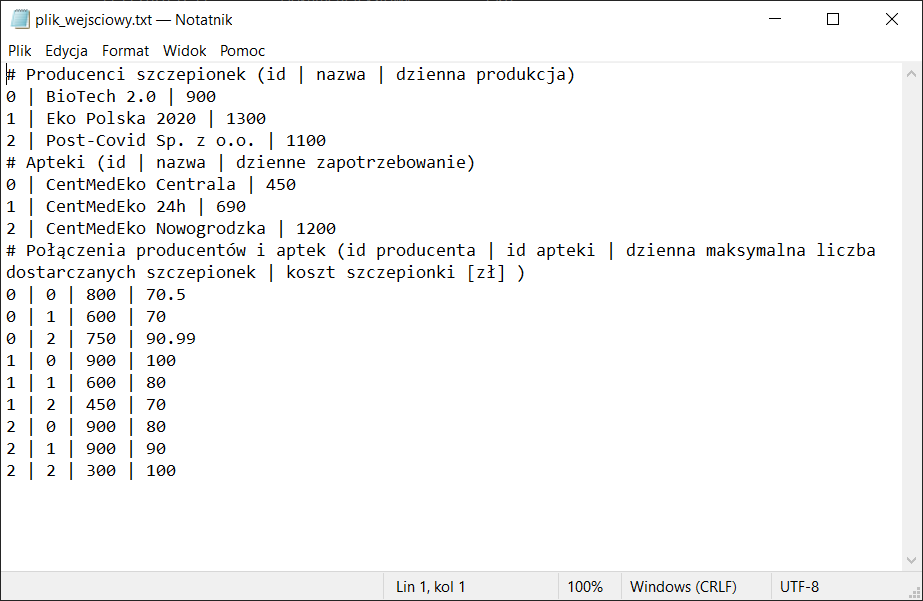
\includegraphics[width=12cm,center]{images/plik_wejsciowy.PNG}
    \captionof{figure}{Przykładowy plik wejściowy}
\end{figure}

\begin{figure} [hbt!]
    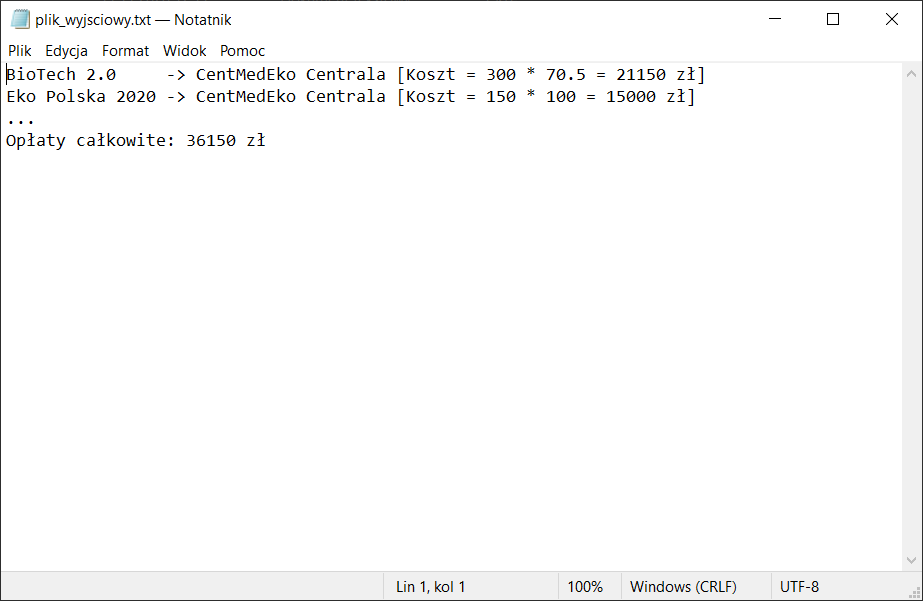
\includegraphics[width=12cm,center]{images/plik_wyjsciowy.PNG}
    \captionof{figure}{Przykładowy plik wyjściowy}
\end{figure}

\clearpage

\subsection{Plik wejściowy - uwagi}
Wszystkie odstępstwa od formatu pliku wejściowego lub błędne wartości będą powodowały \textbf{przerwanie programu}. Po przerwaniu program wypisze \textbf{wiadomość} (na konsolę i do pliku) \textbf{gdzie został popełniony błąd}.

\subsubsection{Wszystkie możliwe odstępstwa od formatu}
\begin{itemize}
    \item ,,Nagłówki'' powinny zostać zachowane (zaczynające się od ,,\#'') i powinny być w jednej linii.
    \item Poszczególne wartości powinny zostać oddzielone sekwencją: ,,spacja'' ,,znak |'' ,,spacja''.
    \item Kolejność ,,sekcji'' w pliku powinna zostać zachowana tzn. najpierw producenci szczepionek, następnie apteki, a na końcu połączenia.
    \item Liczby niecałkowite powinny mieć format ,,Liczba'' ,,znak kropki'' ,,Liczba'' np. 70.5 a nie 70,5.
\end{itemize}

\subsubsection{Jakie są poprawne wartości}
\begin{itemize}
    \item Id producenta ma być liczbą całkowitą nieujemną.
    \item Nazwa nie powinna zawierać znaku ,,|''
    \item Dzienna produkcja powinna być liczbą całkowitą większą od zera.
    \item Dzienne zapotrzebowanie powinno być liczbą całkowitą większą od zera.
    \item Dzienna maksymalna liczba dostarczanych szczepionek powinna być liczbą całkowitą większą od zera.
    \item Koszt szczepionki powinien być liczbą rzeczywistą większą od zera, z dwoma miejscami po przecinku.
\end{itemize}

\section{Scenariusz działania programu}
Jeżeli plik wejściowy będzie źle sformatowany lub będzie posiadał błędną wartość to program przerwie się, a następnie wypisze do pliku i na konsolę informację o błędzie i w której linii pliku on wystąpił.

Jeżeli takich błędów nie będzie to program stworzy plik wyjściowy ,,optymalizacja.txt'' zgodny z formatem pliku wyjściowego.

\section{Źródła}

\begin{itemize}
    \item Tobiasz Siemiński - opis specyfikacji funkcjonalnej: https://sortris.blogspot.com/2010/05/jak-pisac-specyfikacje-funkcjonalna.html
    
    \item Opis problemu przygotował i umieścił na platformie ISOD mgr inż. Paweł Zawadzki
    
\end{itemize}

\end{document}